\documentclass[12pt,fleqn]{article}\usepackage{../common}
\begin{document}


$$ 
c = \frac{ 2c_m}{1 + \cosh |b_c(t-t_{mc})|   }
$$


\begin{minted}[fontsize=\footnotesize]{python}
from scipy.optimize import fmin
import pandas as pd
from numpy.linalg import *
df = pd.read_csv('oil1.csv',sep='\s')
df = df[df['year'] < 2008]

def hubbard_err(w):
    cm=w[0];bc=w[1];tmc=w[2]
    #cm=1;bc=1;tmc=w[2]
    yfit = 2*cm / (1+cosh(bc*(df['year']-tmc)))
    diff = df['oil']-yfit
    e=norm(diff)
    return e

v = fmin(hubbard_err, [2, 2, 1940], maxiter=100000, maxfun=10000)
print v
\end{minted}

\begin{verbatim}
Optimization terminated successfully.
         Current function value: 47.983802
         Iterations: 1460
         Function evaluations: 2523
[  7.82312521e+01  -5.46461718e-02   2.00122099e+03]
\end{verbatim}

\begin{minted}[fontsize=\footnotesize]{python}
df2 = df.set_index('year')
ax = df2['oil'].plot(title='World Oil Production')
ax.set_ylabel("Million Barrels / Year")
plt.savefig('peak_01.png')
\end{minted}




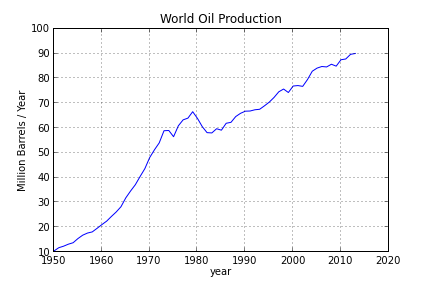
\includegraphics[height=6cm]{peak_01.png}

\url{http://www.earth-policy.org/Updates/2007/Update67_data2.htm#table1}

\url{http://en.wikipedia.org/wiki/Hubbert_curve}

\url{http://www.eia.gov/cfapps/ipdbproject/iedindex3.cfm?tid=5&pid=53&aid=1&cid=ww,&syid=1980&eyid=2013&unit=TBPD}

\url{http://www.countercurrents.org/mushalik270314.htm}


\begin{minted}[fontsize=\footnotesize]{python}
cm=v[0];bc=v[1];tmc=v[2]
def hubbard(x): 
    return 2*cm / (1+cosh(bc*(x-tmc)))
pred = map(hubbard, df['year'])
print pred
\end{minted}

\begin{verbatim}
[16.924388178067382, 17.760322280529234, 18.631227556616846, 19.537889196479689, 20.481032316015906, 21.461311283892353, 22.47929824754776, 23.535470864252485, 24.630199255472636, 25.763732216890215, 26.936182732546801, 28.147512859753753, 29.397518071646875, 30.685811166502461, 32.01180587704831, 33.374700338790234, 34.773460603531355, 36.206804412380087, 37.673185471103409, 39.170778499036672, 40.697465350140497, 42.250822530296425, 43.828110457535445, 45.426264830466863, 47.041890483498179, 48.671258114231854, 50.310304267392148, 51.954634949500878, 53.599533228099332, 55.239971137565227, 56.870626169685266, 58.48590257059648, 60.079957596361105, 61.64673279758766, 63.179990309965397, 64.673354023696504, 66.120355392533526, 67.514483524974992, 68.849239079214911, 70.11819136323507, 71.315037925924187, 72.433665818504394, 73.468213612139152, 74.413133181584215, 75.263250210019208, 76.013822340141232, 76.660593893877405, 77.199846109441864, 77.628441900639373, 77.943864228864243, 78.144247291531642, 78.22839986889646, 78.195820330468578, 78.046702977672183, 77.781935585442525, 77.403088196024541, 76.912393407052377, 76.312718576839288]
\end{verbatim}

\begin{minted}[fontsize=\footnotesize]{python}
df2['pred'] = pred
ax = df2['oil'].plot(); ax.hold(True)
ax = df2['pred'].plot()
plt.savefig('peak_02.png')
\end{minted}

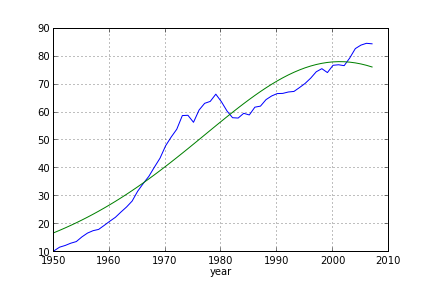
\includegraphics[height=6cm]{peak_02.png}














\end{document}
